\documentclass[tikz, border=10pt]{standalone}

\usepackage{listings}
\usepackage{pgf}
\usepackage{tikz}
\usepackage[utf8]{inputenc}
\usetikzlibrary{arrows,automata}
\usetikzlibrary{positioning}


\tikzset{
    state/.style={
           rectangle,
           rounded corners,
           draw=black, very thick,
           minimum height=2em,
           inner sep=2pt,
           text centered,
           },
}


\begin{document}

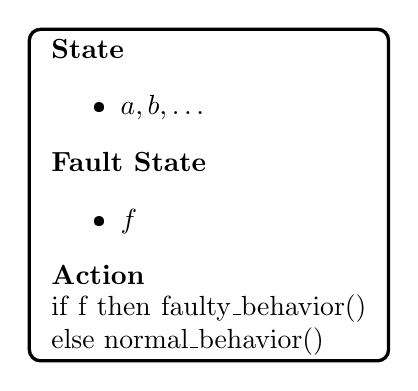
\begin{tikzpicture}[->,>=stealth']

 \node[state] (S)
 {\begin{tabular}{l}
  \textbf{State}\\
  \parbox{4cm}{\begin{itemize}
   \item $a, b, \ldots$
  \end{itemize}
  }\\
  \textbf{Fault State}\\
  \parbox{4cm}{\begin{itemize}
   \item $f$
  \end{itemize}
  }\\
  \textbf{Action}\\
  \parbox{4cm}{if f then faulty\_behavior() else normal\_behavior()}
 \end{tabular}};

\end{tikzpicture}

\end{document}
